%%=============================================================================
%% Methodologie
%%=============================================================================

\chapter{Methodologie}
\label{ch:methodologie}

%% TODO: Hoe ben je te werk gegaan? Verdeel je onderzoek in grote fasen, en
%% licht in elke fase toe welke stappen je gevolgd hebt. Verantwoord waarom je
%% op deze manier te werk gegaan bent. Je moet kunnen aantonen dat je de best
%% mogelijke manier toegepast hebt om een antwoord te vinden op de
%% onderzoeksvraag.

Om zelf de voor- en nadelen zoals die naar voor kwamen uit de literatuurstudie na te gaan werd er een project opgezet in Elasticsearch. In het project werden een aantal data-analyses uitgevoerd worden met als doel een antwoord te krijgen op enkele interessante vragen. Tijdens het opzetten van het project en het uitvoeren van de data-analyses kon er worden bepaald welke voor- en nadelen, die uit de literatuurstudie bleken, echt van toepassing zijn. Daarnaast kwamen ook andere sterktes en zwaktes van Elasticsearch opdagen die aansluiten bij het resultaat van de literatuurstudie.

Een belangrijk aspect van zelf een project opzetten om bepaalde zaken zelf te gaan ondervinden is dat men de grootte van het voor- of nadeel beter kan inschatten. Als men bijvoorbeeld een moeilijkheid van Elasticsearch ondervindt, dan zal men toch nog een antwoord op de vooraf opgestelde vraag willen krijgen. Men zal dan ondervinden in hoeverre Elasticsearch toch in staat is om als hulpmiddel te dienen bij het oplossen van die vraag. Of misschien is er een workaround mogelijk waardoor de zwakte eigenlijk niet zo'n groot probleem is. Dat is informatie die met een literatuurstudie moeilijker te verkrijgen is.

\section{De dataset}
De dataset die gebruikt werd voor het onderzoek is afkomstig van een applicatie van het bedrijf Insites Consulting. Insites Consulting is een consulting bureau die haar klanten ondersteunt in het nemen van belangrijke beslissingen. Dat doet men aan de hand van marktonderzoek. Uit de resultaten van zo'n marktonderzoek creëert men inzichten die worden doorgegeven aan de klant. 

De ervaring leert dat het soms moeilijk is voor de klant om zo'n informatie verstandig te benutten. In andere gevallen komen de resultaten van het marktonderzoek ergens in een documentje op de computer van de klant en wordt er verder niks mee gedaan. Insites Consulting bouwde enkele jaren geleden een applicatie die aan deze problemen zou moeten tegemoet komen. De applicatie heet Insight Activation Studio. Elke klant krijgt een unieke Studio die aangepast wordt aan de noden, waarden en kleuren van de klant. Die aanpassingen gebeuren in eerste instantie door mensen van Insites Consulting maar ook de klant heeft een dashboard ter beschikking. Een dashboard is een geïsoleerd stuk van de applicatie dat admin-gebruikers toelaat om de studio van hun bedrijf te beheren.  

Werknemers van de klant kunnen zich registreren bij de Studio van hun bedrijf. Eens ze aangemeld zijn krijgen ze de mogelijkheid om walls\footnote{Een wall is een verzameling van tiles die min of meer over hetzelfde onderwerp gaan.} en tiles\footnote{Een tile is vergelijkbaar met een post op Facebook maar met meer mogelijkheden. Een tile bestaat onder andere uit een type (idee, filmpje, foto, observatie, quiz, discussie, …), een titel, een beschrijving maar er kunnen ook andere media aan toegevoegd worden. Andere mensen kunnen op jouw tile reageren en kunnen deze ook liken.} aan te maken. Ook krijgen ze walls en tiles van anderen te zien. Het is de bedoeling dat de verworven inzichten op deze Studio komen zodat mensen daarop kunnen reageren en deze eventueel kunnen liken. Zo ziet men snel welke inzichten populairder zijn bij de werknemers en krijgen die bijzondere interesse. Uit die inzichten kunnen ook nieuwe ideën vloeien.

De Insights Academy is een feature die in de Studio verweven zit. Daarop kunnen werknemers lessen volgen om te leren hoe men gebruik kan maken van zo’n inzicht. Daarnaast zijn er nog andere zaken (leaderboards, widgets, teams, … ) die het volledige proces leuker maken. Insights Activation Studio is dus eigenlijk de social media voor werknemers binnen een bedrijf om inzichten te creëren en leven in te blazen.

De dataset die gebruikt werd in dit onderzoek is de SQL Server dataset van de Insight Activation Studio. Een uitleg van de tabellen wordt telkens gegeven wanneer deze van toepassing is. Een script om de dataset te creëren in SQL Server is te vinden in Bijlage 1. \textbf{TODO: BIJLAGE 1 toevoegen} Alle namen van personen die in de dataset voorkomen werden willekeurig gegenereerd om anonimiteit te verzekeren.

\section{De vragen}
De vragen werden opgesteld door Ken Vanderbeken, die Lead Developer is aan de Insight Activation Studio. Voor hem is het zeer interessant om te weten of er aspecten zijn die bepalen of een tile succesvol is. Een tile stelt een inzicht voor en dit tot leven brengen is net de primaire doelstelling van de applicatie. Daarom gaan alle vragen daarover. Om te bepalen of een tile succesvol is wordt er berekend hoeveel likes en comments de tile heeft.

De vragen zijn de volgende:
\begin{itemize}
	\item Werken bepaalde tile types beter dan andere? Meer response? (like/comment) 
	\item Waar gebeuren de meeste likes? Vanaf de homepagina of op wall pages?
	\item Heeft de lengte van de titel van een tile invloed op aantal comments/likes? 
\end{itemize}

\section{Opzetten van het project}

Voor de installatie van Elasticsearch wordt er verwezen naar sectie \ref{Installatie} uit de literatuurstudie waar de installatie aan bod komt. De installatie zou probleemloos moeten kunnen uitgevoerd worden op de manier zoals het daar beschreven staat. Het gebruik van de grafische user interface is onnodig aangezien het over een eenvoudige installatie gaat.

Om de data te exporteren wordt er gekozen voor een tool die ondersteund wordt door de community: JBDC importer for Elasticsearch. De keuze is niet uitgegaan naar Logstash omdat er in de gids vermeld staat dat Logstash vooral gebruikt wordt om logs op te slaan. Ook is er voor dit onderzoek geen nood aan alle features die Logstash te bieden heeft. De methode van de JBDC importer biedt dus alles wat voor dit onderzoek nodig is met de bijhorende simpliciteit.

Bij dit onderzoek werd er gebruikt gemaakt van de JBDC importer versie 2.3.4.1 dat aangeboden wordt als een ZIP bestand. Het uitgepakte bestand bevat een modelscript dat slechts een aantal aanpassingen nodig heeft om uitgevoerd te kunnen worden. Het script laat toe om een query naar de databank te sturen, en de resultaten op te slaan in één van uw Elasticsearch indices. Voor de SQL Server JDBC driver werd versie 6.2 gebruikt. Ook deze wordt als een ZIP bestand aangeboden en moet uitgepakt worden. Het uigepakte bestand wordt vervolgens naar de lib map in de JDBC importer gekopieerd. Deze stap is onnodig indien men met een MySQL databank werkt. 

De voorlaatste stap is het aanmaken van de indices. Een index aanmaken in Elasticsearch is zeer eenvoudig. Via de API moet er een PUT-request worden gestuurd met als URL: http://localhost:9200/naam\textunderscore index.
Per index moet het modelscript, mits een aantal aanpassingen, uitgevoerd worden. Het modelscript is te zien in figuur \ref{fig:data_import}.

\begin{figure}
	\centering
	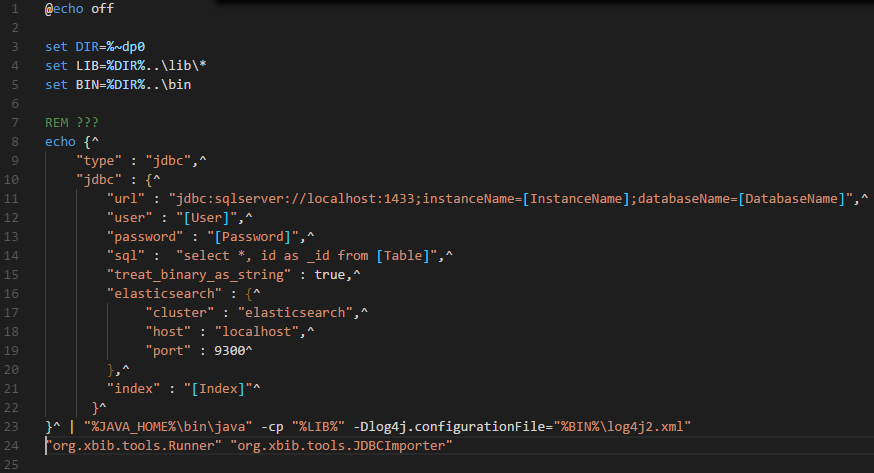
\includegraphics[width= 15cm]{data_import}
	\caption{Modelscript om data te exporteren van SQL Server naar Elasticsearch}
	\label{fig:data_import}
\end{figure}

\section{Uitvoeren van de data-analyses}
Nadat de dataset succesvol werd overgezet is het tijd om met Elasticsearch te leren werken. Het zelf ondervinden van hoe steil de leercurve is van Elasticsearch is namelijk ook een onderdeel in dit onderzoek. \textbf{Een belangrijk pluspunt van de zoek- en analyse machine dat hierbij naar voren kwam}, is dat er veel support is. Op de website wordt een zeer uitgebreide, gestructureerde gids aangeboden die alle mogelijkheden van Elasticsearch overloopt. In de gids kan men ook de versie kiezen waarop men werkt. Op die manier blijft de informatie steeds relevant. De gids wordt goed onderhouden wat wil zeggen dat er steeds informatie over de nieuwste versie van Elasticsearch ter beschikking is. 

\textbf{Om de leercurve zelf aan den lijve te ondervinden is het goed dat men nog geen voorkennis hebben van de taal noch van de structuur die gebruikt wordt om de API van Elasticsearch aan te spreken.}\textbf{ Waar de nieuwe gebruiker doorgaans wel voorkennis van zal hebben} is de query language van SQL Server. Die voorkennis komt goed van pas omdat er vanuit de guides van Elasticsearch\textbf{ vrij regelmatig} verwezen wordt naar de query language van SQL Server. Dat vergemakkelijkt het leerproces. Je zou kunnen stellen dat gebruikers zonder die voorkennis dan sterk benadeeld worden maar de makers van de gids zorgden ervoor dat je ook zonder die voorkennis de verschillende aspecten van Elasticsearch kunt begrijpen. Kennis van de query language van SQL Server geeft dus een boost aan het leerproces maar is zeker \textbf{geen noodzaak}.

Naast de uitstekende gids kan men ook vragen stellen op het forum dat toegankelijk is \textbf{via de website van Elasticsearch}. Op het forum bieden medewerkers van Elasticsearch of andere mensen hun oplossingen aan voor \textbf{eventuele problemen}. Het forum kan als een actief forum beschouwd worden met 907 nieuwe posts per maand. Ook op andere bekende forums is Elasticsearch een populair onderwerp. Een zoekopdracht op Stack Overflow geeft bijna 68 000 resultaten die gerelateerd zijn aan Elasticsearch. Uit de literatuurstudie bleek dat er ook veel boeken ter beschikking zijn. Ze worden door velen sterk aangeraden en kunnen geraadpleegd worden om meer gedetailleerde informatie op te zoeken. 

Hieronder volgt nogmaals een opsomming van de vragen waarop een antwoord \textbf{moest gevonden worden} via Elasticsearch. Bij elke vraag staat beschreven hoe er \textbf{werd} te werk gegaan, welke moeilijkheden er \textbf{zich hebben voorgedaan} en welke \textbf{positieve punten} van Elasticsearch er ondervonden \textbf{werden}. Om de API aan te spreken wordt er gebruik gemaakt van Postman. Elke andere API client zou hiervoor\textbf{ ook dienst kunnen doen}.

\subsection{Werken bepaalde tile types beter dan andere?}
Om een antwoord op deze vraag te vinden hebben we 2 indices uit de dataset nodig: de tile-index en de tiletype-index. Er bestaat een één op veel relatie tussen tile en tiletype. Een tile houdt steeds \textbf{de} id van zijn tiletype bij. \textbf{De tiles moeten eerst gegroepeerd worden per type waarna per groep de gemiddelde activiteit wordt berekend.} Uit de resulaten zal blijken of tiles van een bepaalde tiletype meer activiteit vertonen dan andere. De activiteit wordt beschouwd als de som van het aantal likes en het aantal comments.

Elasticsearch biedt een oplossing voor dit probleem. Met aggregaties wordt het mogelijk om documents te groeperen. In de gids over aggregaties wordt de vergelijking gemaakt met \textbf{de} GROUP BY \textbf{bewerking} in SQL Server. Daarbij \textbf{vermeldt} men dat aggregaties in Elasticsearch echter veel meer mogelijkheden bieden. Zo bestaan er een 50-tal soorten aggregaties. Dat is een groot aantal die het gebruik ervan complex maakt. Zeker omdat aggregaties ook genest kunnen worden. Dat wil zeggen dat men binnen een aggregatie opnieuw een aggregatie kan doen. De flexibiliteit is echter zeer hoog omdat de mogelijkheden enorm zijn. \textbf{Deze ervaring strookt dus niet} met \textbf{TODO: BRON} waarin verteld wordt dat Elasticsearch minder flexibiliteit biedt dan SQL Server. Bij het oplossen van de volgende vraag wordt hierop teruggekomen. \textbf{TODO: BEN JE HIEROP TERUGGEKOMEN?}

Om alle tiles uit de tile-index op te vragen \textbf{moet er} een GET request \textbf{gestuurd worden} naar Elasticsearch. Om verdere filteringen, sorteringen of andere functies uit te voeren zijn er 2 methodes. Bij de eerste methode kan men parameters meegeven op het einde van de URL. Bij de tweede methode kan men een body in JSON-formaat meegeven aan de call. Hier kan voor de tweede methode gekozen worden omdat niet alle mogelijkheden binnen Elasticsearch meegegeven kunnen worden aan de URL. Bij deze keuze wordt er echter meteen \textbf{over} een eerste probleem gestruikeld. Niet alle API clients, inclusief Postman, bieden de mogelijkheid om een body mee te geven aan een GET call omdat dat geen normale manier van werken is. De ontwikkelaars van Elasticsearch hebben daar rekening mee gehouden en zorgden ervoor dat data opvragen ook met een POST request mogelijk is. Aangezien er een kleine workaround is wordt dit niet beschouwd als een nadeel.

De URL van de call ziet er als volgt uit: http://localhost:9200/tile/\textunderscore search. Het woord tile duidt aan dat \textbf{er} binnen de tile-index \textbf{gezocht wordt}. Het woord \textunderscore search geeft aan dat \textbf{er} naar documents binnen de index \textbf{gezocht wordt}. Indien dat laatste niet meegeven \textbf{wordt} krijg je enkel het schema van de index terug.

De body is te zien in figuur \ref{fig:script1}. De eerste parameter in de body is size. Size geeft aan hoeveel documenten er zichtbaar moeten zijn in het resultaat. \textbf{Dit is te} vergelijken met SELECT TOP X in SQL Server. Aggregaties worden telkens onder alle documents getoond. Aangezien \textbf{enkel} de aggregaties \textbf{belangrijk zijn, wordt de size 0} zodat er geen documents zichtbaar zijn. De tweede parameter is de aggregatie. \textbf{De naam hiervan is } group\textunderscore by \textunderscore tileTypeId. In de terms parameter van \textbf{deze} aggregatie \textbf{wordt getoond dat op het veld tileTypeId moet gegroepeerd worden}. Daarna \textbf{wordt een nieuwe aggregatie meegegeven} aan group\textunderscore by \textunderscore tileTypeId. \textbf{Deze aggregatie krijgt de naam} avg\textunderscore response. \textbf{Die aggregatie moet dus een gemiddelde berekenen.} In het script wordt meegegeven van welke waarde het gemiddelde moet worden genomen. \textbf{In dit geval gaat het om het} gemiddelde van de som van het aantal comments en het aantal likes en dat \textbf{wordt op die manier meegegeven}.

\begin{figure}
	\centering
	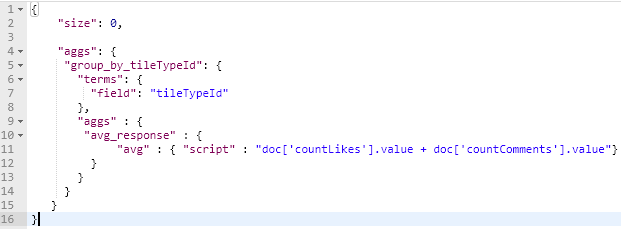
\includegraphics{script1}
	\caption{Body script 1}
	\label{fig:script1}
\end{figure}

\textbf{Het resultaat van het script is te} zien in figuur \ref{fig:scriptresult1}. Elk resultaat begint met wat algemene informatie zoals: hoeveel tijd de query nodig had, hoeveel shards er succesvol overlopen zijn, hoeveel shards faalden, hoeveel documents er voldoen aan de zoekopdracht, etc. In figuur \ref{fig:scriptresult1} is echter enkel het deel te zien dat op dit moment interessant is, namelijk de resultaten van de aggregaties.

\begin{figure}
	\centering
	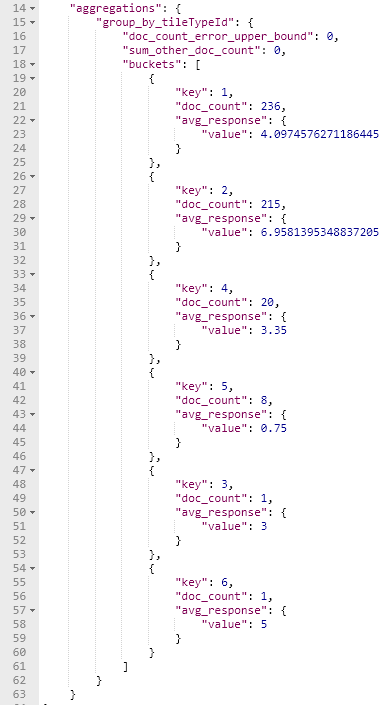
\includegraphics{scriptresult1}
	\caption{Resultaat script 1}
	\label{fig:scriptresult1}
\end{figure}

Het key-veld in de resultaten stelt telkens het tiletypeid voor waarop \textbf{werd gegroepeerd}. Per aggregatie werd er een nieuwe aggregatie uitgevoerd die de gemiddelde activiteit berekende. De gemiddelde activiteit valt af te lezen in het value-veld. Het is duidelijk dat, in deze dataset, tiles met tiletypeid 2 meer activiteit vertonen dan andere tiles. Dat is leuk om te weten maar zegt op zich niet veel.\textbf{Het is vooral belangrijk om te }weten met welk tiletype deze id overeen komt. \textbf{Hierbij wordt echter op een probleem gestoten}.

Om een zoekopdracht uit te voeren op meerdere indices tegelijk zouden de indeces bij bepaalde voorwaarden moeten \textbf{samengevoegd worden}. In SQL Server kan men dit realiseren met het JOIN-sleutelwoord. Join-operaties zijn zeer duur in Elasticsearch. Zo duur dat de ontwikkelaars ervoor zorgden dat join-operaties over verschillende indices onmogelijk zijn. \textbf{?? Is dit echt zo? Heb je hiervoor een bron? Want dit is een "straffe" uitspraak??} Een document moet alle informatie bevatten die nodig is om te beslissen of het al dan niet in de zoekresultaten terechtkomt. Je moet dus op voorhand beslissen hoe je gaat zoeken en \textbf{de} index daaraan aanpassen. Indien de query herhaaldelijk moet worden uitgevoerd is dat de moeite waard en vormt dat geen probleem. Maar in \textbf{dit} geval \textbf{moet er een  éénmalig antwoord komen op deze vraag}. \textbf{Dat impliceert dat er telkens een nieuwe index moet aangemaakt worden en dat de data opnieuw moet geïmporteerd worden} om er nadien slecht één query op uit te voeren. Die manier van werken zorgt voor een index overhead en wordt in dit onderzoek ervaren als een groot nadeel van Elasticsearch.

Bij deze vraag \textbf{is er echter slechts één tiletype interessant}. \textbf{Een andere mogelijkheid is om een tweede query uit te voeren op de tiletype-index. Door het meegeven van de id kan het juiste tiletype opgevraagd worden.} Deze manier van werken heeft als voordeel dat \textbf{er geen nieuwe index moet aangemaakt worden}. De nadelen van deze manier van werken zijn dat je telkens meerdere queries moet uitvoeren en dat het niet altijd realistisch is om dat te doen. Wanneer \textbf{het tientallen documenten zou betreffen} dan gaat de voorkeur toch naar het aanmaken van een nieuwe index. Voor deze vraag is dat niet van toepassing dus wordt er voor de tweede methode gekozen.

\textbf{Er wordt een query aangemaakt} met URL: http://localhost:9200/tiletype/\textunderscore search. De body van de query is te zien in figuur \ref{fig:script2}. Er wordt simpelweg gezocht naar een document met id 2. In het resultaat (figuur \ref{fig:scriptresult2}) \textbf{is te zien dat er gesproken wordt een tiletype idea.} 

Het antwoord op de eerste vraag luidt: Ja, tiles met tiletype idea werken beter dan andere.

\begin{figure}
	\centering
	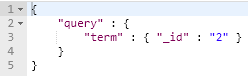
\includegraphics{script2}
	\caption{Body script 2}
	\label{fig:script2}
\end{figure}

\begin{figure}
	\centering
	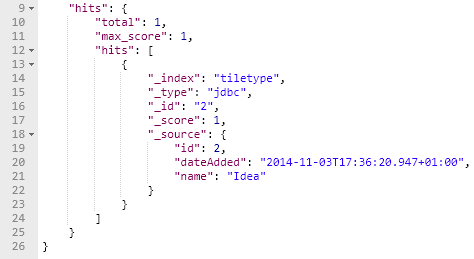
\includegraphics{scriptresult2}
	\caption{Resultaat script 2}
	\label{fig:scriptresult2}
\end{figure}

\subsection{Waar gebeuren de meeste likes? Vanaf de homepagina of op wall pages?}
Om deze vraag te beantwoorden \textbf{zijn er} 3 indices nodig: like, log en logtype. Wanneer een gebruiker naar de homepagina navigeert dan wordt dat gelogd in de log-tabel met logtype 8. Wanneer een gebruiker naar een wall page navigeert dan wordt dat gelogd in de log-tabel met logtype 10. Wanneer een gebruiker een tile liked dan komt er een nieuw record in de like tabel. Bij dit probleem \textbf{is het wel nodig} om een nieuwe index aan te maken. \textbf{De 3 tabellen moeten worden samengenomen en alle documents zijn noodzakelijk.} 

In \textbf{deze} nieuwe index \textbf{zijn er} slechts twee velden nodig: de id van de like en de pagina waarop de like gebeurde. Er zal een script moeten geschreven worden om de data van SQL Server naar de nieuwe index te exporteren. In het script moet, per like, uitgemaakt worden of die vanop de homepagina of vanop een wall pagina gebeurde. \textbf{Er wordt dus gezocht} naar de meest recente log met logtype 8 of 10 die minder recent is dan de like en dezelfde userId heeft als de gebruiker die de like uitvoerde. Het SQL-script is te zien in figuur \ref{fig:script3}. Het valt op dat sommige likes dubbel voorkomen in de index. De \textbf{oorzaak} hiervan is dat de tijd waarop een log aangemaakt wordt, telkens afgerond is op één minuut. Als men binnen de minuut beide pagina's bezoekt en vervolgens een tile liked is het niet duidelijk vanop welke pagina de like gebeurde. Omdat het hier om een zeer klein aantal dubbele likes gaat worden deze gewoon meegeteld op beide pagina's.

\begin{figure}
	\centering
	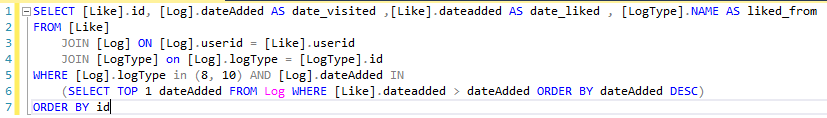
\includegraphics[width=17.5cm]{script3}
	\caption{SQL-script voor het importeren van de data uit vraag 2}
	\label{fig:script3}
\end{figure}

De index staat klaar en nu \textbf{moet er} enkel nog een aggregatie \textbf{gedaan worden} op de plaats waar er geliked werd. De URL van de query ziet er als volgt uit: http://localhost:9200/question2/\textunderscore search. In de body (figuur \ref{fig:script4}) \textbf{wordt er meegegeven dat er een aggregatie moet gebeuren} op het liked\textunderscore from-veld. Aan de hand van die aggregatie \textbf{is te} zien hoeveel likes er op de homepagina gebeurden en hoeveel likes er op wall pages gebeurden. Het resultaat van de query \textbf{wordt getoond} in figuur \ref{fig:scriptresult4}.

\begin{figure}
	\centering
	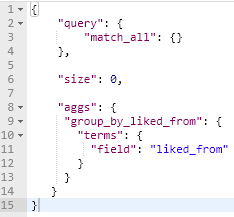
\includegraphics{script4}
	\caption{Body script 4}
	\label{fig:script4}
\end{figure}

\begin{figure}
	\centering
	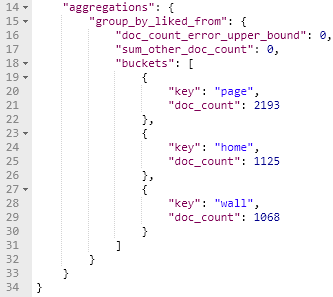
\includegraphics{scriptresult4}
	\caption{Resultaat script 4}
	\label{fig:scriptresult4}
\end{figure}

Uit het resultaat \textbf{is af te leiden} dat de meeste likes vanaf de homepagina gebeuren. Dat is dan ook meteen het antwoord op de vraag. Men kan echter wel zien dat het aantal likes vanaf de homepagina en het aantal likes vanaf wall pages zeer dicht bij elkaar liggen. 

Bij het oplossen van deze vraag zou het onbegonnen werk zijn geweest om meerdere queries uit te voeren op verschillende indices. De werkwijze die in de vorige vraag de voorkeur kreeg kon hier niet worden herbruikt. Het meest complexe rekenwerk was het bepalen vanop welke pagina een like gebeurde. Elasticsearch biedt geen eenvoudige manier om die berekening te doen. Het gebrek aan joins werd nu ervaren als een groot nadeel.

\subsection{Heeft de lengte van de titel van een tile invloed op aantal comments/likes}

Om te bepalen of er een verband is tussen de variabelen lengte van de titel en aantal comments/likes \textbf{zal} een chi-kwadraat toets \textbf{uitgevoerd worden}. Indien uit het resultaat blijkt dat er een verband is kan de sterkte van het verband berekend worden met Cramers V. Elasticsearch biedt geen ondersteuning voor dergelijke berekeningen. Deze kunnen nochtans zeer interessant zijn bij het maken van een data-analyse. Om toch een antwoord op de vraag te krijgen zullen we Elasticsearch als hulpmiddel gebruiken bij het uitvoeren van de chi-kwadraattoets. Op die manier zal het duidelijk worden in hoeverre Elasticsearch kan helpen bij ingewikkelde calculaties zoals de chi-kwadraat toets. 

De eerste stap bij het uitvoeren van een chi-kwadraat toets is het opstellen van een kruistabel. Bij het opstellen van een kruistabel moeten \textbf{de variabelen ingedeeld worden} in klassen. \textbf{Per variabele wordt de grootste waarde in de dataset berekend zodat bepaald wordt tot hoever de klassen moeten reiken.} Figuur \ref{fig:calculatenamelength} toont hoe de lengte van de langste naam van een tile \textbf{kan berekend worden}. Bij het uitvoeren van deze query krijgt men \textbf{een} resultaat van 49. \textbf{Aan de hand van} een gelijkaardige query \textbf{werd gevonden} dat de maximale som van het aantal likes en het aantal comments van een tile 33 is.

\textbf{Op basis van het voorgaande wordt ervoor gekozen om de variabelen op te delen in drie klassen.} Voor de variabele lengte van de titel stellen de klassen [0, 17], [18, 34] en [35, 51] respectievelijk 'korte titel', 'middellange titel' en 'lange titel' voor. Voor de variabele aantal comments/likes stellen de klassen [0, 11], [12, 22] en [23, 33] respectievelijk 'weinig activiteit', 'gemiddelde activiteit' en 'veel activiteit' voor.\textbf{De kruistabel kan nu opgesteld worden.}

\begin{figure}
	\centering
	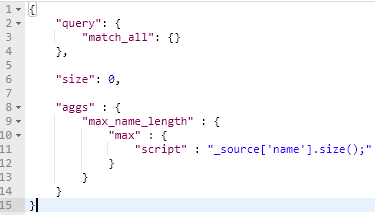
\includegraphics{calculate_name_length}
	\caption{Body om de lengte van de langste naaam van een tile te berekenen}
	\label{fig:calculatenamelength}
\end{figure}

Er kan een query geschreven worden in Elasticsearch die de waarden voor \textbf{deze} kruistabel teruggeeft. De aggregatie die aangemaakt \textbf{wordt} is terug te vinden in bijlage 2. \textbf{TODO: voeg bijlage 2 toe} \textbf{De aggregatie krijgt de naam table ???.} In het filter-veld \textbf{wordt '1=1' meegegeven}  om te forceren dat alle documents in de resultaten terugkomen. Het filter-veld zou hier als overbodig kunnen worden beschouwd maar het weglaten ervan zorgt voor foutmeldingen. \textbf{In de table-aggregatie worden er drie nieuwe aggregaties aangemaakt.} Elk van de aggregaties stelt een klasse van de lengte van de titel voor. \textbf{De aggregaties krijgen respectievelijk de namen} row0-17, row18-35 en row\textbf{35-51}. In het filter-veld van elk van deze aggregaties \textbf{wordt meegegeven} dat enkel documents die tot die klasse behoren mogen meegeteld worden in de resultaten. \textbf{Dit gebeurt door} restricties op te leggen op de lengte van de titel van de tile. In elk van de drie aggregaties \textbf{zijn er} opnieuw drie aggregaties die de klassen van het aantal comments/likes voorstellen. Opnieuw \textbf{worden er restricties meegegeven} in elk van de filter-velden zodat de juiste documents in de juiste klassen komen. Het resultaat van de query wordt weergegeven in bijlage 3 \textbf{TODO: voeg bijlage 3 toe}. In figuur \ref{fig:tablewrong} worden de resultaten in een kruistabel weergegeven.

De tweede stap houdt in \textbf{dat} er voor elke waarde in de kruistabel een verwachte waarde moet berekend worden. De verwachte waarde wordt berekend door het totaal van de rij te vermenigvuldigen met het totaal van de kolom en dat resultaat te delen door de echte waarde. De verwachte resultaten komen opnieuw in een kruistabel (figuur \ref{fig:tablewrongV}).

In de derde stap wordt er gevalideerd of de verwachte waarden voldoen aan de stelling van Cochran. De stelling van Cochran luidt dat geen enkele cel een verwachte waarde kleiner dan 1 mag hebben. Daarnaast mag niet meer dan 20\% van de cellen een verwachte waarde kleiner dan 5 hebben. Indien de kruistabel niet voldoet aan de stelling van Cochran dan heeft de uitkomst van de chi-kwadraat toets geen betekenis. \textbf{De kruistabel wordt gevalideerd} aan de stelling van Cochran en \textbf{er blijkt} dat meer dan 20\% van de cellen een verwachte waarde kleiner dan 5 heeft. Om de chi-kwadraat toets toch te kunnen uitvoeren zullen de klassen moeten opnieuw ingedeeld moeten worden. De klassen van de lengte van de titel \textbf{worden behouden}. De nieuwe klassen [0, 16] en [17, 33] stellen respectievelijk 'weinig activiteit' en 'veel activiteit' voor. \textbf{De query wordt aangepast} om de waarden voor de kruistabel te berekenen. De nieuwe query is terug te vinden in bijlage 3 \textbf{TODO: voeg bijlage 3 toe}. In figuur \ref{fig:tablecorrect} worden de resultaten in een kruistabel weergegeven.


\begin{figure}
	\centering
	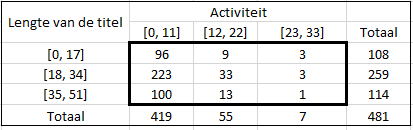
\includegraphics{table_wrong}
	\caption{Kruistabel voor vraag 3}
	\label{fig:tablewrong}
\end{figure}

\begin{figure}
	\centering
	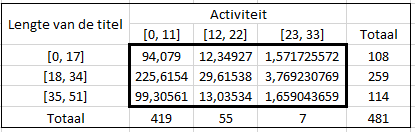
\includegraphics{table_wrong_V}
	\caption{Verwachte waarden voor vraag 3}
	\label{fig:tablewrongV}
\end{figure}

\begin{figure}
	\centering
	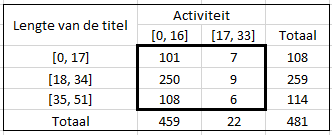
\includegraphics{table_correct}
	\caption{Kruistabel voor vraag 3 na de herindeling van de klassen}
	\label{fig:tablecorrect}
\end{figure}

\textbf{De verwachte waarden worden opnieuw berekend } (figuur \ref{fig:tablecorrectV}) en \textbf{de kruistabel wordt opnieuw gevalideerd} aan de stelling van Cochran. Alle cellen hebben een verwachte waarde groter of gelijk aan 1. Slechts 1/6 (16,667\%) van de cellen hebben een verwachte waarde die kleiner is dan 5. Deze keer wordt er voldaan aan de stelling van Cochran. Het resultaat van de chi-kwadraattoets zal nu wel betekenisvol zijn.


\begin{figure}
	\centering
	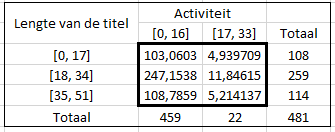
\includegraphics{table_correct_V}
	\caption{Verwachte waarden voor vraag 3 na de herindeling van de klassen}
	\label{fig:tablecorrectV}
\end{figure}

In de vierde en laatste stap \textbf{wordt} de waarde voor $\tilde\chi^2$ (chi-kwadraat) \textbf{berekend}. Deze waarde \textbf{kan vergeleken worden} met de kritieke waarde om te bepalen of er samenhang is tussen de twee variabelen. $\tilde\chi^2$ is de som van de kwadraten van het verschil van de werkelijke waarde en de verwachte waarde gedeeld door de verwachte waarde. In een laatste kruistabel (figuur \ref{fig:table_correct_values}) \textbf{is} deze waarde voor elke cel \textbf{terug te vinden}.

\begin{figure}
	\centering
	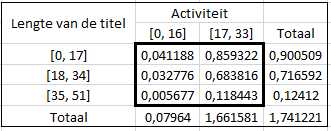
\includegraphics{table_correct_values}
	\caption{Verwachte waarden voor vraag 3 na de herindeling van de klassen}
	\label{fig:tablecorrectvalues}
\end{figure}

De som van al deze waarden, en daarmee ook $\tilde\chi^2$, is 1,7412. \textbf{Het} significantieniveau \textbf{bedraagt} 5\%. Om de kritieke waarde op te zoeken \textbf{zijn een} aantal vrijheidsgraden (df) nodig. Het aantal vrijheidsgraden bereken je door het aantal rijen - 1 te vermenigvuldigen met het aantal kolommen  -1. In dit geval is dat 2 keer 1. De kritieke waarde voor 2 vrijheidsgraden met significantieniveau 5\% is 5,99. De berekende $\tilde\chi^2$ is strikt kleiner dan 5,99 wat wil zeggen dat er geen verband is tussen de twee variabelen.

